\chapter{RAUFlow}
\label{Capítulo 5}

% **************************** Define Graphics Path **************************
\ifpdf
    \graphicspath{{Chapter5/Figs/Raster/}{Chapter5/Figs/PDF/}{Chapter5/Figs/}}
\else
    \graphicspath{{Chapter5/Figs/Vector/}{Chapter5/Figs/}}
\fi

En cap\'itulos anteriores se ha detallado las caracter\'isticas m\'as importantes del prototipo y sus componentes. 
Resta detallar el dise\~no de la aplicaci\'on RAUFlow, encargada de implementar el plano de control del prototipo. Por ello en el presente cap\'itulo se propone un an\'alisis de dicha componente, siguiendo un proceso de dise\~no tradicional de Ingenier\'ia de Software, dividido en 4 etapas. Una primera etapa de an\'alisis de requerimientos, una segunda etapa de relevamiento de casos de uso, una tercera etapa de dise\~no del modelo de datos, y finalmente una cuarta etapa para el dise\~no general de la arquitectura de la aplicaci\'on. Ademas se presentan los aspectos m\'as importantes relacionados a la implementaci\'on de RAUFlow como por ejemplo las implementaciones del algoritmo de ruteo din\'amico y del algoritmo de distribución de etiquetas, como se implementa QoS entre otros detalles. 

\section[An\'alisi de requerimientos]{An\'alisis de requerimientos}

Anteriormente en la sección ~\ref{3.1} se definieron algunos de los requerimientos relevados para el prototipo de la RAU2. De ellos y de un trabajo de an\'alisis sobre la realidad modelada se desprende la siguiente tabla de requerimientos para RauFlow:

\clearpage
\begin{table}[Htl]\centering
\begin{tabularx}{\textwidth}{|>{\setlength\hsize{1.0\hsize}\setlength\linewidth{\hsize}}X|}
\hline
Requerimientos Funcionales\\ \hline
\hline
\begin{itemize}
\item El Sistema debe de proveer la facilidad para obtener la informaci\'on asociada a cada nodo de la red, permitiendo a su vez agregar informaci\'on que facilite la identificaci\'on del mismo para un usuario.
\item El Sistema debe proveer la facilidad para agregar, modificar y eliminar redes virtuales. 
%En particular al trabajar con redes virtuales y sus datos, se debe soportar el manejo de datos como la numeraci\'on IP del tr\'afico asociado a una red virtual, informaci\'on de capa de transporte, entre otros.
\item El Sistema debe proveer la facilidad para obtener toda la informaci\'on relevante de una red virtual.
\item El Sistema debe permitir visualizar de alguna forma los caminos constru\'idos para encaminar el tr\'afico de una red virtual en particular, a trav\'es de la red del protot\'ipo.
\item El Sistema debe proveer la facilidad para visualizar el estado de las tablas de flujos asociadas a cualquier nodo de la red del protot\'ipo.
\end{itemize}\\
\hline
\end{tabularx}
\end{table}

\begin{table}[Htl]\centering
\begin{tabularx}{\textwidth}{|>{\setlength\hsize{1.0\hsize}\setlength\linewidth{\hsize}}X|}
\hline
Requerimientos no Funcionales\\ \hline
\hline
\begin{itemize}
\item Se debe utilizar siempre que sea posible herramientas de software libre y c\'odigo abierto.
\end{itemize}\\
\hline
\end{tabularx}
\end{table}

Teniendo en cuenta la descripci\'on del problema y los requerimientos anteriores, se procedio con el modelado de la realidad. Los resultados obtenidos se presentan en la siguiente secci\'on.

%Teniendo en cuenta los requerimientos anteriores, se procede con el relevamiento de los casos de uso. Los resultados obtenidos se presentan en la siguiente secci\'on.

\section[Modelado de la realidad]{Modelado de la realidad}

A continuaci\'on (ver figura ~\ref{fig:ModeloDeDatos}), se expone el modelo de datos utilizado para representar a la realidad.\\

En el mismo se destacan en color amarillo las clases utilizadas para representar la topolog\'ia de la red y sus elementos(Nodos, Interfaces y Enlaces). Cabe destacar sobre estas tres clases que en la representaci\'on asumida, se busca modelar la topolog\'ia como un multigrafo dirigido. Esto se debe a que:

\begin{enumerate}
\item Tradicionalmente se utilizan grafos para el modelado de una topolog\'ia de red, siendo una representaci\'on sencilla y clara.

\item En MPLS un camino o mejor llamado LSP tiene sentido, permitiendo por ejemplo asegurar un valor de ancho de banda en un enlace para un sentido y un valor diferente para el otro sentido. Adem\'as permite establecer caminos diferentes para el tr\'afico en un sentido y en otro, priorizando por ejemplo el tr\'afico  en uno de los sentidos al utilizar el mejor camino. Utilizando grafos dirigidos puede modelarse este comportamiento.

\item En la pr\'actica nada impide que dos equipos o nodos est\'en conectados por m\'as de un enlace. De hecho este escenario es bastante beneficioso para asegurar conectividad ante la falla de enlaces. Utilizando multigrafos este escenario es modelado de forma clara.
  
\end{enumerate}

\begin{figure}[ht!] 
\centering    
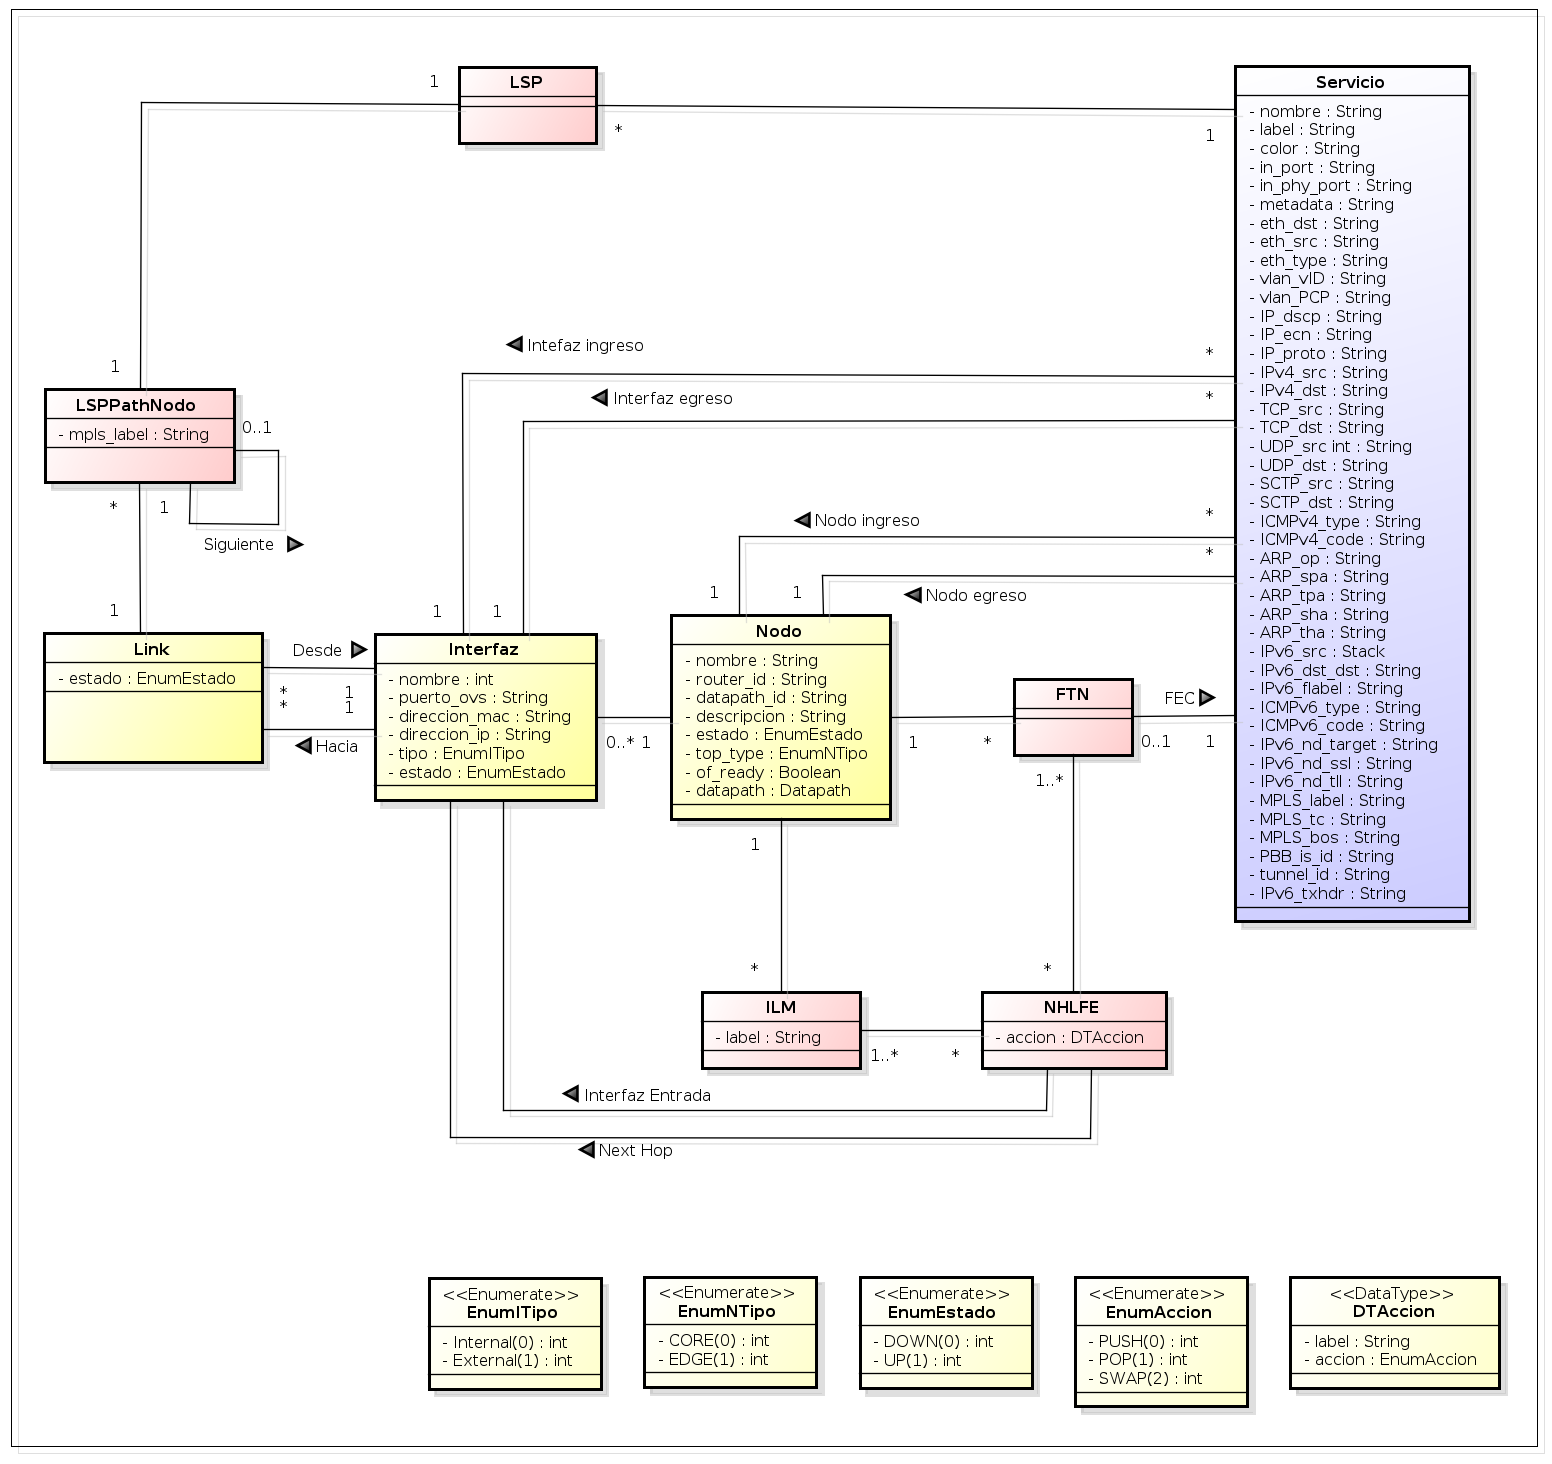
\includegraphics[width=1\textwidth]{DiagramaClases}
\caption[Modelo de datos]{Modelo de datos}
\label{fig:ModeloDeDatos}
\end{figure}

En un mulrigrafo dirigido se tienen nodos y aristas con sentido; siendo representados los nodos de una red por los nodos del grafo y los enlaces entre estos por las aristas.

En el modelo planteado(el cual a su vez esta orientado a objetos), se incorpora un tercer concepto;  las interfaces de un nodo. Desde entonces dos nodos presentan una arista si cada uno esta asociado a una instancia de la clase Interfaz y existe una instancia de la clase Link asociada a ambas interfaces, mediante las relaciones “Desde” y “Hacia”; indicando adem\'as estas el sentido del link.

Cabe destacar adem\'as, que en el modelo planteado no se asume que un Nodo sea f\'isicamente un dispositivo RAU-Switch; solamente se asume por simplicidad del modelo que sea un dispositivo de capa tres. Con esto se intenta contemplar la posibilidad de incorporar en un futuro adem\'as de nodos construidos en base al diseño de RAU-Switch, nodos implementados por ejemplo en base a hardware comercial.\\
  
[No se si explicar la cardinalidad 1 - * de las Interfaces - Link, la cual esta dada asi por la situacion switch dentro del core]\\

En la figura ~\ref{fig:ModeloDeDatos} se presenta el modelo de dominio realizado a partir de la realidad planteada. En el mismo se destacan en color amarillo aquellas entidades que se entiende se corresponden al modelado de los elementos de la topolog\'ia como lo son Nodos e Interfaces. Por otro lado en rosado se destacan aquellas entidades relacionadas al concepto MPLS que se consideran importantes, como lo son las tablas FTN, ILM y NHLFE. Finalmente vale la pena destacar el concepto de Servicio, con el cual se decidi\'o representar los servicios de VPN. Vale la pena destacar que en el modelo planteado para modelar diferentes clasificaciones de trafico para una misma VPN, se consideran varias instancias de Servicio, una para cada clasificación de tr\'afico. 

%Interesa destacar adem\'as del concepto de Servicio, que es una redefinici\'on desde una visi\'on centralizada del concepto FEC en la teor\'ia de MPLS, concepto que en la literatura de MPLS tradicional esta vinculado a un solo nodo en una red, y no a muchos como se propone en este trabajo.  


Sobre este modelo de dominio se trabaj\'o hasta llegar finalmente al diagrama de clase de dise\~no que se presenta a continuaci\'on en la figura [ref].\\

Teniendo en cuenta los requerimientos mencionados, y el modelado de la realidad presentado, se procede con el relevamiento de los casos de uso. Los resultados obtenidos se presentan en la siguiente secci\'on.

\section[Relevamiento de casos de uso]{Relevamiento de casos de uso}

La lista de casos de uso presentada a continuaci\'on se corresponde con un conjunto de funcionalidades b\'asicas, que permiten la exploraci\'on de la potencialidad del enfoque SDN aplicado al problema planteado. 

\begin{itemize}
\item Listar Servicios
\item Agregar Servicio
\item Modificar Servicio
\item Eliminar Servicio
\item Ver Topolog\'ia
\item Ver informaci\'on b\'asica Nodo
\item Ver tabla de Flujos Nodo
\item Filtrar Lsps
\item Editar Informaci\'on extra Nodo
\item Editar Informaci\'on extra Interfaz
\end{itemize}

%De esta forma quedan presentados los requerimientos relevados sobre RauFlow, el modelado de la realidad, y los casos de uso relevados. Resta entonces presentar un esbozo de la arquitectura de la aplicaci\'on RauFlow, para que el lector finalmente este en condiciones de comprender el dise\~'no del prototipo en su totoalidad.
\section[Arquitectura de RauFlow]{Arquitectura de RauFlow}

En esta secci\'on se presenta la arquitectura de la aplicación RauFlow(ver figura ~\ref{fig:VistaComponentes2}), profundizándose en el funcionamiento de sus principales componentes.\\

Como se muestra en la figura\ref{fig:VistaComponentes2}, RauFlow esta basado principalmente en una aplicaci\'on Ryu(RauFlowApp) y un conjunto de aplicaciones Ryu adicionales.\\ 

Con el objetivo de mantener simple y modular el dise\~no de RauFlow, se implementa en RauFlowApp solamente aquellas funcionalidades y responsabilidades asociadas al protocolo OpenFlow y sus respectivos eventos. Luego responsabilidades y funcionalidades asociadas a la realidad modelada y sus reglas de negocios, son delegadas a una capa de negocios. Ademas se tiene un conjunto de aplicaciones Ryu dise\~nadas e implementadas por terceros, las cuales se encuentran dentro del conjunto de aplicaciones que vienen con el software Ryu. M\'as adelante se explicar\'a en detalle cual es el rol que cumplen estas aplicaciones en el dise\~no de RauFlow.

Para completar esta visi\'on general de RauFlow, se incluye en su arquitectura una interfaz de usuario gr\'afica.\\ 

En res\'umen, el dise\~no de RauFlow se caracteriza por una arquitectura en cuatro capas: (1) capa de presentación, (2) capa de aplicaciones Ryu, (3) capa de negocios, y (4) capa de dispositivos.\\

\newpage
\begin{figure}[ht!] 
\centering    
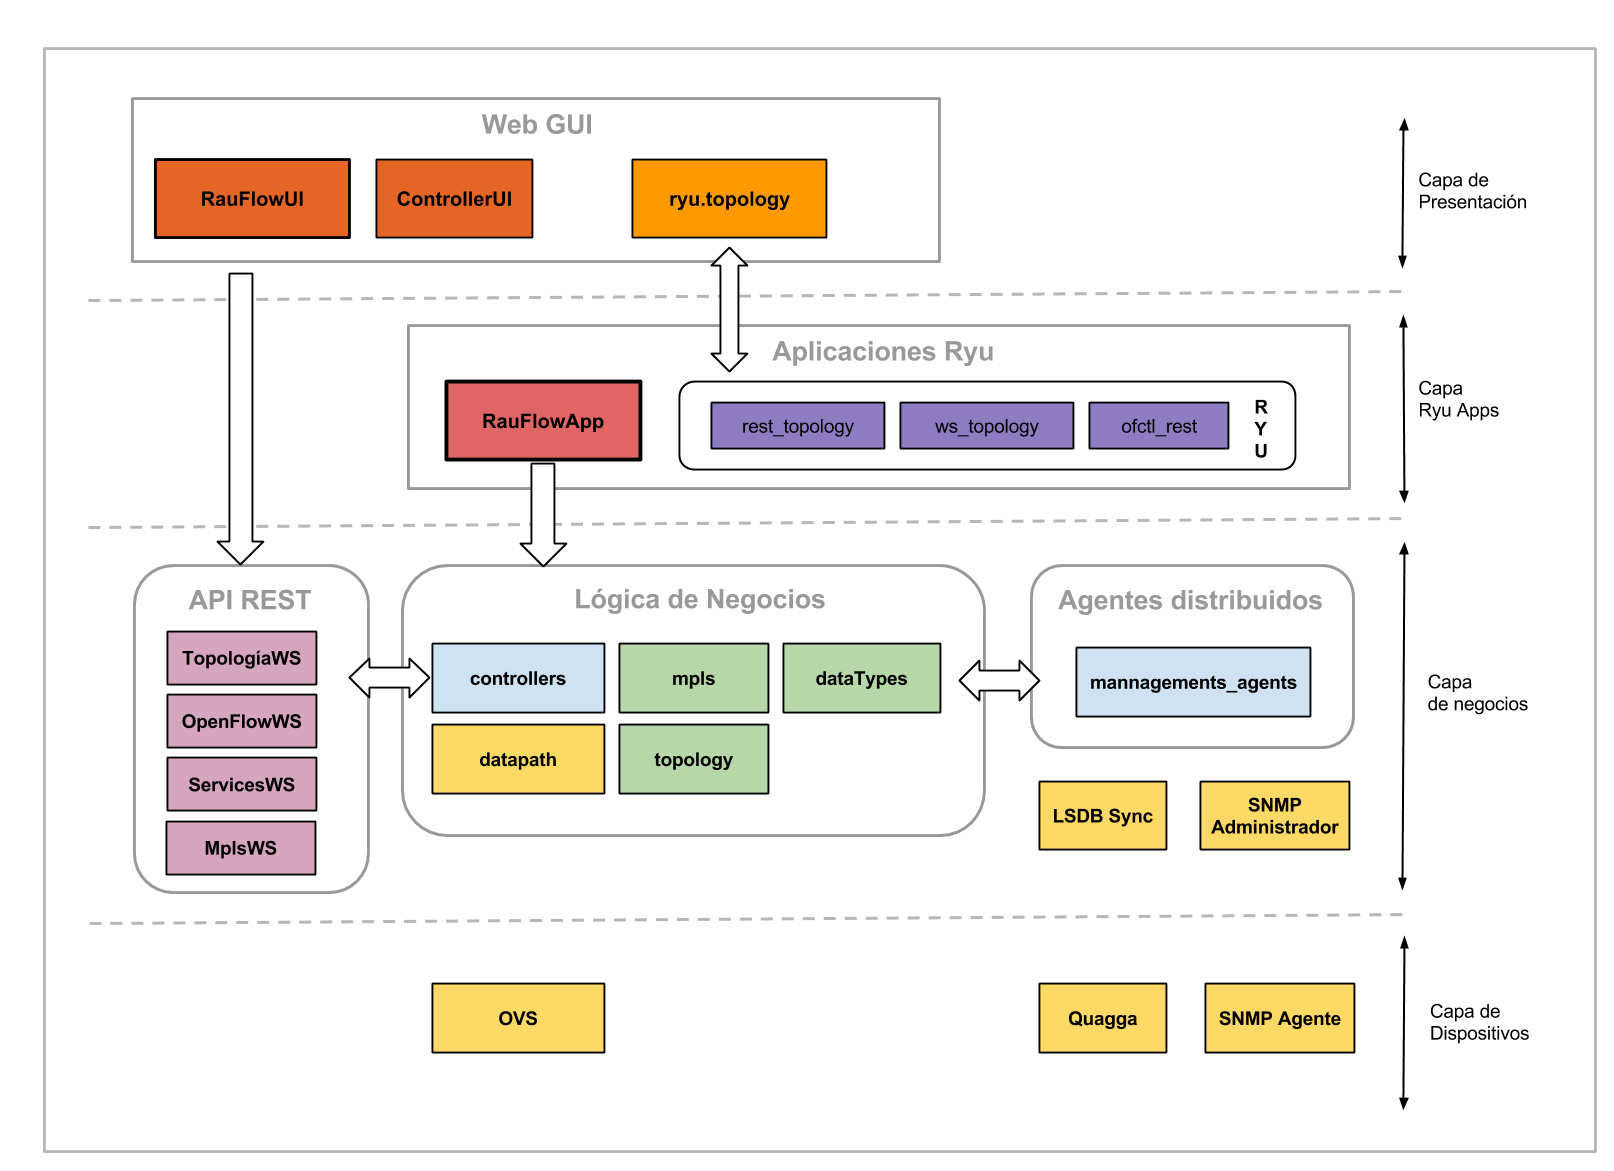
\includegraphics[width=1.0\textwidth]{Disenio_Figure3}
\caption[Vista l\'ogica]{Vista l\'ogica}
\label{fig:VistaComponentes2}
\end{figure}

\subsection{Capa de aplicaciones Ryu}
En esta capa se encuentran las diferentes aplicaciones Ryu que conforman al prototipo. Como se menciona anteriormente, RauFlow esta compuesto por una aplicaci\'on de autoria propia, y tres aplicaciones de terceros(incluidas en las aplicaciones que vienen con el software de controlador).\\

La aplicaci\'on RauFlowApp es la encargada de implementar el plano de control en el prototipo; por lo tanto, a priori su alcance puede ser tan grande como el propio alcance de RauFlow. Esto redunda en una complejidad mayor en el dise\~no de la misma. Por esta razón se decide desacoplar las reglas de negocio de la realidad, de dicha aplicación. De esta forma se genera la mencionada capa de negocios; en donde se coloca todo este conocimiento de la realidad modelada, reglas de negocio, y funcionalidades.  

\subsubsection{Aplicaciones de terceros}
Ryu incluye tres aplicaciones dise\~nadas para implementar una interfaz gr\'afica. Dicha interfaz consiste en un p\'agina web implementada sobre html, javascript y web sockets, que permite visualizar la red en su totalidad. Estos son los dispositivos del datapath con sus interfaces, y los enlaces existentes.

Por esta razon se incluyen en el dise\~no del proptotipo dichas aplicaciones, agregando funcionalidades  a la capa de presentaci\'on, y reutilizando desarrollos existentes.

\subsection{Capa de Negocios}
La capa de negocios presenta tres componentes bien definidas: una componente de reglas y l\'ogica de negocios de la realidad, una API REST de servicios para el acceso y la manipulaci\'on de datos relacionados a la primera componente, y una tercera componente denominada Agentes distribu\'idos.

\subsubsection{Lógica de Negocios}
La componente lógica de negocios se subdivide en diferentes m\'odulos que agrupan funcionalidades acorde a su naturaleza y responsabilidades. Vale la pena destacar a su vez que cada uno de estos m\'odulos se corresponde en la implementaci\'on con un package en la nomenclatura de Python. Estas funcionalidades y responsabilidades se corresponden de la siguiente forma:

\begin{itemize}
\item \textbf{controller:} Este m\'odulo agrupa diferentes controladores de objetos. Actualmente contiene un \'unico controlador façade, responsable de mantener el \'unico punto de acceso a la las componentes de la l\'ogica de negocios. Contiene desde la implementaci\'on de funciones para dar de alta Servicios, crear LSPs, obtener el mejor camino entre dos nodos de la red, etc.

\item \textbf{topology:} Agrupa las definiciones de objetos utilizados para representar la topolog\'ia como las clases Nodo, Interfaz y Link, así como otros conceptos de la realidad.
 
\item \textbf{mpls:} Contiene las definiciones de los conceptos FTN, ILM, NHLFE(rectificar esto xq esta en topology actualmente), as\'i como el conceptos de Servicio ya explicado anteriormente, y de LSP(label switched path).

\item \textbf{dataTypes:} Mantiene representaciones reducidas de los principales objetos definidos en todos los m\'odulos de la componente de negocios, para el intercambio de datos con por ejemplo la capa de presentaci\'on. 

\item \textbf{datapath:} Agrupa funcionalidades para el acceso al datapath de OpenFlow, como funciones para agregar y eliminar flujos en un switch, u obtener estad\'isticas de una tabla de flujos.
\end{itemize} 

\subsubsection{API REST de servicios}
La componente de Servicios REST, se encuentra subdividida en varios m\'odulos respondiendo al criterio utilizado para el dise\~no modular de la componente de l\'ogica de negocios. [De repente podemos poner como anexo la especificacion de la api para que se vean las funcionalidades que tiene].

\subsubsection{Agentes distribuidos}
Esta componente es la encargada de la interacci\'on con diferentes agentes y procesos instalados en cada router opensource a través de un canal de comunicación IP. Este m\'odulo de comunicaci\'on, as\'i como los diferentes agentes instalados en cada router opensource, juegan un rol irreemplazable en la obtenci\'on de informaci\'on adicional sobre cada nodo; puesto que a partir del canal de comunicaci\'on OpenFlow solamente es accesible Open vSwitch y la informaci\'on contemplada por el protocolo OpenFlow.

Dentro de esta componente, en el diagrama se muestra un modulo denominado \textbf{managements\_ agents}. Este m\'odulo opera como una interfaz de conexi\'on entre los diferentes m\'odulos de la l\'ogica de negocios, y los diferentes m\'odulos que implementan la comunicaci\'on con su respectivo agente distribu\'ido.

En la figura ~\ref{fig:VistaComponentes2} se muestran el modulo \textbf{SNMP Management}, responsable de  la comunicaci\'on con un agente SNMP distribu\'ido entre los nodos del prototipo, con el fin de obtener informaci\'on extra acerca de las interfaces de red de cada router opensource.\\

\subsection{Capa de Presentación}
Dentro de la capa de presentaci\'on se destacan: (1) una interfaz gr\'afica identificada en el esquema como RauFlowUI, la cual implementa cada uno de los casos de uso mencionados anteriormente en [link a la secci\'on de casos de uso], (2) ControladorUI, componente que funciona como nexo entre las funcionalidades de RauFlowUI y la API Rest de Servicios, y (3) \textbf{ryu.topology}. Esta \'ultima componente forma parte del conjunto de apliaciones Ryu adicionales que se incluyen en el dise\~no de RauFlow, y tiene como principal funci\'on la de proveer una representaci\'on gr\'afica en tiempo real de la topolog\'ia existente en el prototipo.\\

\section[Implementaci\'on]{Implementaci\'on}

En esta secci\'on se presentan los aspectos m\'as importantes en relaci\'on a la implementaci\'on de RauFlow. Entre ellos se destacan la presentaci\'on del algoritmo de ruteo din\'amico implementado, el algoritmo de distribusi\'on de etiquetas, las convenciones utilizadas para identificar y crear clases de servicios, entre otros.\\

\subsection{Implementación de Servicio}

En la realidad modelada se tienen dos conceptos fundamentales asociados a una red privada virtual (VPN): (1) el concepto de servicio y (2) el concepto de calidad de servicio.

\begin{enumerate}
\item El concepto de servicio establece un trato diferencial para el tr\'afico asociado a una VPN, bajo ciertas condiciones bien definidas(tipicamente temporales). 
\item El concepto de calidad de servicio (QoS), establece características sobre el procesamiento del trafico en la red(tipicamente reserva de ancho de banda) que repercuten luego en el calculo del camino a seguir por dicho trafico.
\end{enumerate}

En relación al concepto de servicio, en la perspectiva que se adopta en RauFlow presenta las siguientes  características:

\begin{itemize}
\item Es un concepto global que involucra a toda la topolog\'ia
\item Queda determinado parcialmente por la cuádrupla 
\begin{center}
(nodo\_ingreso, interfaz\_ingreso, nodo\_egreso, interfaz\_egreso)
\end{center}
\item Interesa distinguir servicios utilizando las capacidades provistas por los matching fields de OpenFlow 
\item Esta definido temporalmente (para un rango horario espec\'ifico)[esto no se si lo ponemos]
\end{itemize}

De esta forma el concepto de servicio se define mediante la clase Servicio como se muestra a continuación.

\begin{python}
class Service(object):

		#General attributes
		ID 				    #str(uuid.uuid4()) Unique ID 
		name 				#Service name for clear 
							#identification by RauFlow users
							
		lsps				#List of services lsps
		
		ingress_node		#Ingress node of service traffic 
							#in the core
							
		egress_node 		#Egress node of service traffic 
							#in the core
							
		ingress_interface 	#Ingress interface of the service 
							#traffic in the ingress node
							
		egress_interface 	#Egress interface of the service 
							#traffic in the egress node
        
		#Attributes from OFv1.3 matching fields
		in_port			# Switch input port.
		in_phy_port 	# Switch physical input port. 
		metadata 		# Metadata passed between tables. 
		eth_dst 		# Ethernet destination address.
		eth_src 		# Ethernet source address. 
		eth_type 		# Ethernet frame type. 
		vlan_vID 		# VLAN id. 
		vlan_PCP		# VLAN priority. 
		IP_dscp 		# IP DSCP (6 bits in ToS field). 
		IP_ecn  		# IP ECN (2 bits in ToS field). 
		IP_proto		# IP protocol. 
		IPv4_src 		# IPv4 source address. 
		IPv4_dst 		# IPv4 destination address. 
		TCP_src 		# TCP source port. 
		TCP_dst 		# TCP destination port. 
		UDP_src 		# UDP source port. 
		UDP_dst 		# UDP destination port. 
		SCTP_src 		# SCTP source port. 
		SCTP_dst 		# SCTP destination port. 
		ICMPv4_type 	# ICMP type. 
		ICMPv4_code 	# ICMP code. 
		ARP_op			# ARP opcode. 
		ARP_spa 		# ARP source IPv4 address. 
		ARP_tpa 		# ARP target IPv4 address. 
		ARP_sha 		# ARP source hardware address. 
		ARP_tha 		# ARP target hardware address. 
		IPv6_src 		# IPv6 source address. 
		IPv6_dst 		# IPv6 destination address. 
		IPv6_flabel 	# IPv6 Flow Label 
		ICMPv6_type 	# ICMPv6 type. 
		ICMPv6_code 	# ICMPv6 code. 
		IPv6_nd_target 	# Target address for ND. 
		IPv6_nd_ssl 	# Source link-layer for ND. 
		IPv6_nd_tll  	# Target link-layer for ND. 
		MPLS_label 		# MPLS label. 
		MPLS_tc 		# MPLS TC. 
		MPLS_bos		# MPLS BoS bit. 
		PBB_is_id 		# PBB I-SID. */
		tunnel_id 		# Logical Port Metadata. 
		IPv6_txhdr 		# IPv6 Extension Header pseudo-field 
		
\end{python}

En cuanto a como se implementan las nociones de calidad de servicio, se detallan m\'as adelante en~\ref{5.5.4} 

\subsection{Algoritmo de distribución de etiquetas}
Tradicionalmente, en mpls se utilizan etiquetas para: (a) asociar trafico a una VPN en particular y (b) encaminar trafico en la red(reenvío en base a etiquetas). De esta forma se tienen dos niveles de etiquetas: un primer nivel(inner label) utilizado para asociar el trafico con la VPN y asi por ejemplo aplicar localmente políticas de QoS, y el segundo nivel (outer label) utilizado para construir el LSP(label switched path).\\

Para la distribución de etiquetas(inner y outer label) existen protocolos entre los cuales se puede destacar LDP(Label Distribution Protocol)~\citep{LDPRFC}. No obstante estos se encuentran definidos en base a una visión local de un nodo. Por tanto en RauFlow se redefine e implementa un algoritmo para la distribución de etiquetas con una visión global de la red.\\

Asignar etiquetas a VPNs es un problema bastante simple. Una  solución posible es utilizar una variable para iterar sobre un espacio de etiquetas disponibles, y utilizarla secuencialmente.  

Por otro lado asignar etiquetas a un camino mpls, es un problema mas complejo. Aprovechando la visión global de la red, puede redefinirse este algoritmo de distribución de etiquetas de varias formas. En este trabajo se sugieren las siguientes:

\begin{enumerate}
\item Utilizar una variable para iterar sobre un espacio de etiquetas disponibles, y utilizarla secuencialmente. De esta forma no existen dos LSPs en el sistema con etiquetas en com\'un. Esta solución tiene como ventajas su simplicidad y bajo costo en el computo del algoritmo. Por otro lado tiene como desventaja que consume el espacio de etiquetas disponibles(hay que considerar la escala del prototipo).

\item Utilizar una variable para iterar sobre un espacio de etiquetas disponibles para cada puerto asociado a un nodo de la red y por el cual pasa el LSP; cuidando a su vez que no se repitan etiquetas en el camino. De esta forma se permiten caminos con etiquetas repetidas pero dado un link(pares <nodo, puerto> origen y destino), no existen dos LSP con la misma etiqueta asignada a un mismo link. Esta estrategia es bastante mas elaborada que la anterior, pero presenta como principal ventaja que es austera en el consumo de etiquetas. Por otro lado es similar a la estrategia utilizada por el protocolo LDP[revisar si es LDP o QuaggaLDP capaz q es muy fuerte decir solo LDP].
\end{enumerate}

Notese, en relación a la segunda alternativa de implementaci\'on, que debido a la forma en que se distribuyen las etiquetas cada LSP es único; debido a que queda determinado de forma única por la sucesión de links y etiquetas. 

Esto permite, creando un LSP por cada Servicio, prescindir del primer nivel de etiquetas(inner label), puesto que basándose solamente en la etiqueta que trae el paquete y por el puerto de que nodo ingreso, se puede determinar lo que tradicionalmente se conoce como FEC. Esta estrategia presenta como ventajas menos costo de procesamiento de etiquetas en cada nodo, y un aumento del MTU del paquete.\\

RauFlow implementa la segunda alternativa como protocolo para la distribución de etiquetas. El pseudocodigo de este algoritmo se presenta a continuación.\\

\begin{python}
def get_path_mpls_labels(self, path):

    mpls_path = []

    if len(path) == 0:
        #There is not path betwen nodes
        print 'NO path found'

    elif len(path) == 1:
        #If path have only one hop, them the lsp is empty becouse first node is penultimate hop
        mpls_path.append(None)
        
    else:
        #We asign labels for mpls path secuencialy starting on the lowest label value
        label_base = self.MPLS_LABEL_SPACE_MIN
        
        #We separates ultimate hop
        for l in path[:-1]:
        	       
           	#Gets avaiable label
           	label = self.get_avaiable_mpls_label_for_interface(l, label_base)

          	#Add label to lsp
           	mpls_path.append(label)

           	#Increments mpls label_base
            label_base = increment_hex_value(label_base)

            #The penultimate hop remove all mpls labels, then the last link has not asociated label
            mpls_path.append(None)

    return mpls_path
\end{python}

\begin{algorithm}[H]

 \SetKwFunction{obtenerEtiquetasLSP}{obtenerEtiquetasLSP} 
 \SetKwFunction{obtenerEtiquetaParaInterfaz}{obtenerEtiquetaParaInterfaz}
 \SetKwProg{myalg}{Function}{}{}
 \myalg{\obtenerEtiquetasLSP(path){}}{
    Declare MPLS\_LABEL\_SPACE\_MIN $\gets 10$\\
 	Declare mplsPath[]\\
 	Declare labelBase\\
 
	\uIf{len(path) = 1}{
    	$mplsPath \gets mplsPath \cup \{None\}$ \Comment{If path have only one hop, them the lsp is empty becouse first node is penultimate  hop}
 	}
 	\Else{
    	labelBase = MPLS\_LABEL\_SPACE\_MIN \Comment{We asign labels for mpls path secuencialy starting on the lowest label value}
    
   		\ForEach{l in path}{
			label $\gets$ \obtenerEtiquetaParaInterfaz(l, labelBase) \Comment{Gets avaiable label}\\
			
			$mplsPath \gets mplsPath \cup \{label\}$\Comment{Add label to lsp}\\
			
			$labelBase \gets labelBase + 1$\Comment{Increments mpls label base}\\
			
			$mplsPath \gets mplsPath \cup \{None\}$\Comment{The penultimate hop remove all mpls labels, then last link has not asociated label}\\
				
 		}
 	}        
 
 	\Return{mplsPath[]}\;
 
 }
 
 \SetKwProg{myalg}{Function}{}{}
 \myalg{\obtenerEtiquetaParaInterfaz(enlace, etiqueta){}}{
	Completar.. 
 }
 
 \caption{How to write algorithms}
\end{algorithm}

\subsection{Clasificación de trafico}
En la literatura de MPLS, tradicionalmente se utiliza el concepto de FEC(fordwarding equivalence class) para definir un conjunto de paquetes a ser tratados en forma similar(por ejemplo para aplicar QoS). Sin embargo este concepto es desde una visi\'on local a un único nodo.\\

En RauFlow se redefine este concepto, desde la visi\'on global del plano de control.

\subsection{Implementaci\'on de QoS}
\label{5.5.4}

\subsection{Algoritmos de rueto}

\subsubsection{SPF}

\subsubsection{CSPF}
Dijkstra para multi grafos dirigidos.

[AYUDA MEMORIA: Cosas de las que hay que hablar]

\begin{python}

def MultiDijkstra(G, start, end):
    '''
    docs
    '''

    D = {}  # dictionary of final distances
    P = {}  # dictionary of predecessors
    S = {}  # Dictionary with processed nodes
    g_minu_s = {}

    #Inicializa G/S como G
    for g in G:
        g_minu_s[g.router_id] = g

    #Stars processing start node
    S[start.router_id] = start
    g_minu_s.pop(start.router_id) 
    for i in G:
        if(G[start].has_key(i)):
            #They are adjacents so we get the minimum weight link between them
            print 'start: ' + start.router_id + ', end: ' + i.router_id
            link = get_nodes_min_cost_link(start, i)
            D[i] = link.weight
            #P[i.router_id] = {'node': start, 'interface': link.from_node_int}
            P[i] = link 

    #Process nodes untill S has all nodes in G
    for i in range(1, len(G)):
       
        w = select_min_cost_adj_node(g_minu_s, D)
        print w.router_id
        S[w.router_id] = w
        g_minu_s.pop(w.router_id)

        for v in g_minu_s.itervalues():
            l = get_nodes_min_cost_link(w,v)
            print 'Info: start=' + start.router_id + ' end=' + end.router_id 
            print 'v='+ v.router_id + ', D[w]=' + str(D[w]) + ', l.weight='+ str(l.weight) + ', D[v]' + str(D[v])

            if D[w] + l.weight < D[v]:
                D[v] = D[w] + l.weight
                #P[v.router_id] = {'node': w, 'interface': link.from_node_int}
                P[v] = l

    return (D,P)
}


def shortestPathMultiGraph(G, start, end):
    """
    Find a single shortest path from the given start vertex
    to the given end vertex.
    The input has the same conventions as Dijkstra().
    The output is a list of the vertices in order along
    the shortest path.
    """

    Path = []
    
    #Sanity check
    if G.has_key(start) and G.has_key(end):

        D,P = MultiDijkstra(G,start,end)

        i = end
        while i != start:
            l = P[i]
            Path.append(l)
            i = l.from_node_int.node
            
        Path.reverse()

    return Path
\end{python}



\begin{itemize}
\item SPF y CSPF: Mostrar el pseudo codigo del algoritmo de ruteo implementado, mencionar que esta construido sobre dijkstra para multigrafos. En particular mencionar que cosas de QoS interesaria meter en este algoritmo para garrantizar QoS despues en RauFlow

\item Mencionar como se implementaria QoS en RauFlow

\item Capaz algo sobre la interfaz 
\end{itemize}